\documentclass{article}

\usepackage{times}
\usepackage{uist}
\usepackage{graphicx}

\begin{document}

% --- Copyright notice ---
\conferenceinfo{UIST'08}{October 19--22, 2008, Monterey, CA, USA.}
\CopyrightYear{2008}
\crdata{x-xxxxx-xxx-x/xx/xxxx}

% Uncomment the following line to hide the copyright notice
% \toappear{}
% ------------------------

\bibliographystyle{plain}

\title{HoverCross: Seamless Diagram Creation and Editing for Pen-Based
       Interfaces}

%%
%% Note on formatting authors at different institutions, as shown below:
%% Change width arg (currently 7cm) to parbox commands as needed to
%% accommodate widest lines, taking care not to overflow the 17.8cm line width.
%% Add or delete parboxes for additional authors at different institutions. 
%% If additional authors won't fit in one row, you can add a "\\"  at the
%% end of a parbox's closing "}" to have the next parbox start a new row.
%% Be sure NOT to put any blank lines between parbox commands!
%%

\author{
\parbox[t]{7cm}{\centering
	     {\em Alice Zhu}\\
	     Harvey Mudd College\\
             Claremont, CA\\
	     xzhu@hmc.edu}
\parbox[t]{7cm}{\centering
	     {\em Christine Alvarado}\\
	     Harvey Mudd College\\
	     Claremont, CA\\
	     alvarado@cs.hmc.edu}
}

\maketitle

\abstract A central problem in pen-based interfaces is how to
transition smoothly between drawing and editing. Separate drawing and
editing modes can be awkward and distracting, while modeless editing
gestures are error-prone. We present HoverCross, a seamless inking and
editing interface that provides a simple and reliable method for users
to create and edit drawings without explicit mode changes.  HoverCross
combines the strengths of several recent developments in pen-based
interfaces.  With HoverCross, users ink normally and then select
objects or ink strokes by crossing over them in the hover space above
the tablet screen.  They can then edit their selection through a
context menu on the canvas.  The results of our user study indicate
that HoverCross provides an efficient, fluid and robust transition
between drawing and editing.  Furthermore, over half of our
participants prefer HoverCross over existing interfaces for several
common diagram creation and editing tasks.

\classification{H5.2 [Information interfaces and presentation]:
User Interfaces. - Graphical user interfaces.}

\terms{Design, Human Factors}

\keywords{Hover space, pen input, tablets.}

\tolerance=400 
  % makes some lines with lots of white space, but 	
  % tends to prevent words from sticking out in the margin

\section{INTRODUCTION}

The promise of pen-based interfaces is that they provide a natural way
for users to create diagrams and take free-form notes.  However, the
integration of diagram creation and diagram editing remains a barrier
to the widespread use of these interfaces.  Pens are more convenient
and natural for drawing, but editing with a pen remains cumbersome
when the user is forced to rely on graphical user interfaces designed
for a mouse and keyboard.  Because the user must use the pen for both
drawing and editing (or suffer the inconvenience of switching between
the pen and the keyboard), a core challenge for pen-based computing is
to construct an interface that allows users to switch easily between
the two tasks, while allowing the system to unambiguously interpret a
given pen stroke as drawing or editing.

Recent years have brought many proposed solutions to this problem.
Traditional solutions (e.g., Windows Journal) require the user to
enter ``edit mode,'' usually by pressing a software button.  This
solution is simple, but the problems with modes are well
known~\cite{Tesler1981Smalltalk}.  Using hardware buttons (e.g., the
bezel buttons on the side of the Tablet PC) to trigger mode switching
helps solve these issues because the mode switch is temporary---as
soon as the user releases the button, the interface reverts to drawing
mode.  Thus, there is little potential for mode confusion.  Studies
suggest that this approach can be quite effective and
natural~\cite{Li2005Experimental,Hinckley2006Springboard}.  However,
simply pressing the button requires not only extra physical effort,
but in many cases also an extra hand.

Other researchers take a recognition-based
approach~\cite{Saund2003Stylus,Zeleznik2006Fluid}, attempting to distinguish
automatically between drawing and editing strokes (e.g., lasso
selections or gestures).  However, even with choice
mediators~\cite{Mankoff2000Providing} to help resolve recognition
ambiguities, recognition errors can be confusing.  Furthermore, as we
argue below, it is not clear that lasso selection is optimal for many
selection tasks.

Recently, researchers have explored using the hover space\footnote{The
\textit{hover space} is the space above the surface of a digital
tablet where the pen is still tracked but does not generate ink or
mouse events.} to invoke editing commands.  Grossman et al. present
Hover Widgets~\cite{Grossman2006Hover}, in which the user performs
gestures in the hover space to activate editing menus.  Following on
this work, Subramanian et al. explore the possibility of using several
layers of the hover space to perform different editing
tasks~\cite{Subramanian2006Multilayer}, while Kattinakere et
al. formally model users' ability to track (e.g., execute gestures) in
hover space \cite{Kattinakere2007Modeling}.


While each of these recently developed approaches brings us closer to
the dream of seamless pen-based drawing and editing, we believe our
arsenal of drawing and editing techniques is not yet complete.
Specifically, for common diagram creation and editing tasks, Hover
Widgets or a multi-level hover space solution may be too heavyweight.

We explore the power and simplicity that can be obtained by combining
the simplest aspects of many existing techniques.  Our interface,
called HoverCross, combines the strengths of hover space editing,
crossing-based selection (e.g.,~\cite{Apitz2004Crossy}), and simple
gesture-triggered context menus (e.g.,~\cite{Hinckley2005Design}),
resulting in an interface that is trivial to learn, reliable, and fast
for common drawing and editing tasks.  Furthermore, our
approach integrates seamlessly with almost any other pen-based editing
technique, so in the worst case users can simply ignore it and fall
back on traditional editing methods.

%% Advantages of our approach: Simple, easy to learn, relatively little
%% chance of recognition error, integrates seamlessly with other
%% techniques, powerful (preferred by some users and faster than other
%% techniques for some common tasks).

%% Our interface provides
%% only one simple, reliably recognized gesture for the user to remember,
%% and this gesture is performed on the canvas so the user does not need
%% to learn to make it in hover space.  \textit{This paragraph is key and
%% needs some work.  The main contributions are that the hover space is
%% not overloaded so you don't need to use gestures in it.  Selection is
%% the number one thing you want to do in editing, and in effect it is a
%% precursor to all other editing things, so you just have to provide
%% support for that, and then you can leverage the fact that when
%% something is selected the user is probably editing.}  

%% I took this text out, but I want it around because it's nicely
%% phrased and I may have lost some of it when I wrote the text above.

%% We propose a new interface not only for creating and manipulating
%% objects with a stylus, but also for transitioning seamlessly between
%% the two tasks. Our work builds on and combines several existing
%% ideas. First, Grossman et al. explore the hover space  for diagram
%% editing [2]. We propose using this space to trigger selection reliably
%% and conveniently. To perform selection in the hover space, we use a
%% crossing metaphor, explored in CrossY, [3] as a substitute for the
%% traditional point-and-click interaction. To manipulate the selection,
%% we use a simple gesture performed on the Tablet screen to bring up a
%% ring-shaped menu around the location of the pen, as described in
%% Scriboli [4].


\section{INTERACTION USING HOVERCROSS}

In many modal pen-based interfaces (e.g., Windows Journal), it is
\textit{selection}, not editing in general, that is typically
relegated to its own mode.  This division makes sense, as selecting
objects in a drawing is typically the first step in performing almost
any editing task.  Once the user selects an object, she can edit it
via a menu or direct manipulation.  An explicit selection mode seems
necessary because any apparent selection stroke just as easily could
be a drawing stroke.

The key insight behind HoverCross is that relegating the process of
selection to the hover space allows users to switch seamlessly between
drawing and selecting without pressing any buttons.  Furthermore,
because the user performs only selection in the hover space, a simple
crossing interface suffices, and there is no need to perform gestures
in the hover space.  The system then leverages the context of the
selection to give the user additional power through a
gesture-invoked context menu or direct interaction with the selected
objects.

In our interface, the user draws normally on the screen to create
diagrams containing simple shapes and text.  The diagrams and text the
user draws currently are recognized by the Microsoft gesture and text
recognition engines, but HoverCross also works with unrecognized ink.
Below we explain our motivation for recognizing the users' ink.


To edit the diagram, the user hovers the pen briefly over the tablet
to trigger selection. The brief pause prevents triggering selection
every time the stylus enters the range, as it inevitably does on its
way to the screen. Once selection is triggered, a small vertical line
appears in the middle of each object (Figure~\ref{fig:handles}), and
the user simply needs to cross the stylus over the line in either
direction in hover space to select the object; crossing the line again
deselects it.  Figure~\ref{fig:contextMenu} shows selected
objects. The user easily can cross over multiple objects to select all
of them.  To clear the selection, the user moves the pen in hover
space off the edge of the screen.

Using the hover space for selection is particularly convenient for
cluttered diagrams in which the user wishes to edit several objects
separated by intervening shapes or text.  The user can enter the hover
space to cross one object and then immediately exit the hover space by
moving the pen tip away from the screen.  The selected object remains
selected even when the pen is outside of hover space.  To select
another object, the user simply needs to re-enter hover space near
that object.

\begin{figure}[tb]
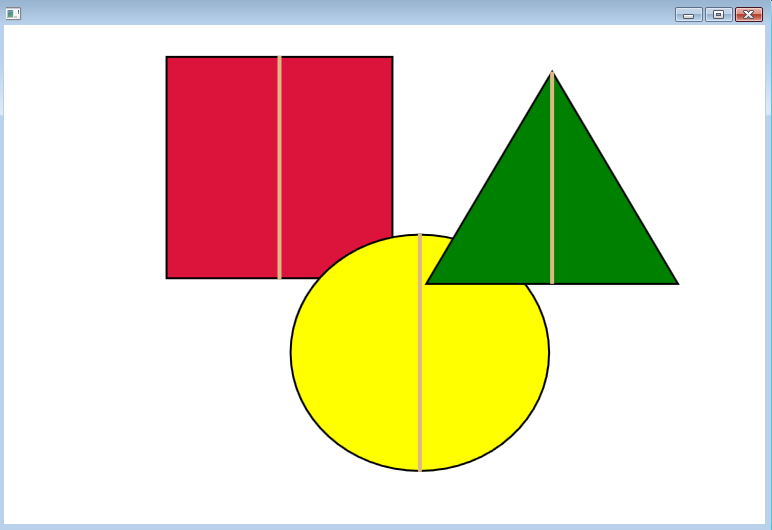
\includegraphics[width=3.0in]{SelectionHandlesOn}
\caption{Vertical bars appear in each shape to give users a crossing
  target.} 
\label{fig:handles}
\end{figure}

%% \begin{figure}[tb]
%% 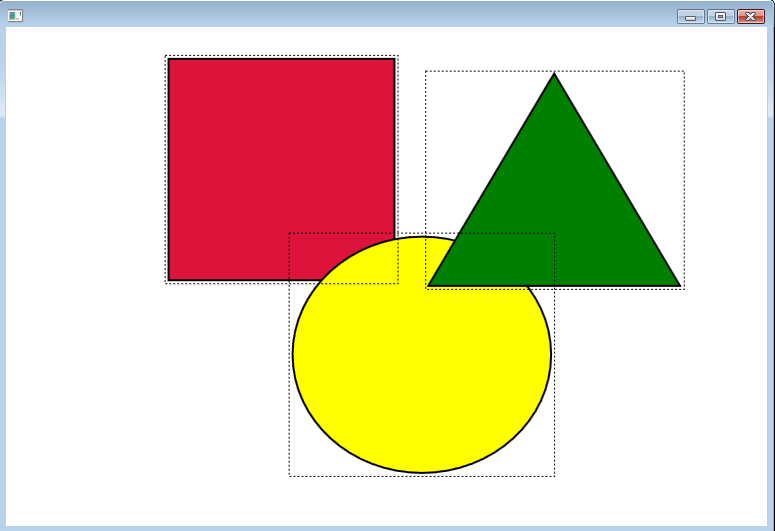
\includegraphics[width=3.0in]{SelectedObjects}
%% \caption{How selected objects appear when the user is outside of hover
%% range (either with the pen down or away from the screen).} 
%% \label{fig:selection}
%% \end{figure}


Once the user has selected at least one item, she can either edit the
selected item, or continue to draw new portions of the diagram.  The
user has several options for editing the diagram.  She can move
selected shapes by dragging one of them with her pen on the
screen. As long as she does not cross the handle in hover space,
touching the shape will not deselect it.  For more complicated
editing tasks, the user can draw a simple gesture (an arc to the
right) anywhere on the screen to bring up a ring-shaped context menu
around the tip of the stylus (Figure~\ref{fig:contextMenu}).  The
content of the menu depends on the type of objects selected, such
as text or shapes. Another short movement allows the user quickly to
choose from the given options to manipulate the selection. With little
practice, the user easily can coordinate drawing, selecting, and
editing in one fluid motion.

\begin{figure}[tb]
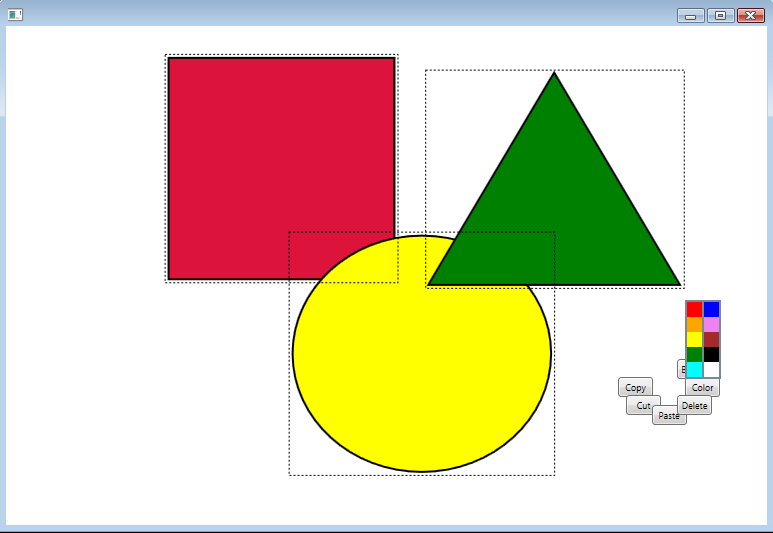
\includegraphics[width=3.0in]{ColorMenu}
\caption{The context menu that appears when the user makes a simple
  gesture.  The menu appears at the tip of the stylus at the end of
  the gesture, and actions apply to all selected shapes.}
\label{fig:contextMenu}
\end{figure}

The HoverCross technique is appropriate for any application that
combines pen-based drawing and editing.  Our example application
supports the creation of clean diagrams that combine shapes and text,
such as might be produced in PowerPoint or Visio.  We chose this
domain because creating polished diagrams typically requires more
intensive editing than simply drawing freeform notes and diagrams. In
a previous pilot study in which we observed people creating slides in
PowerPoint, we found that they relied heavily on copying, pasting,
resizing and moving shapes within their diagrams.  This domain thus
allows us to evaluate the utility of HoverCross for its intended
purpose.

In many ways, our HoverCross interface is incredibly simple, yet quite
powerful.  First, because drawing and selection take place in two
distinct spaces, there can be no ambiguity about the user's
intent. Second, users learn only one simple gesture.  Although our
gesture is so simple it could conceivably be confused with drawing
strokes, it would be straightforward to construct a gesture that is
rarely confused with drawing strokes, such as one of the compound
gestures in~\cite{Laviola2004MathPad}.  Users perform the gesture on
the screen, so there are no issues of learning to execute more complex
gestures in hover space.  Third, the context-specific in-place menus
allow the user easily to access the most common editing commands.

Confirming previous results~\cite{Apitz2004Crossy}, the crossing
selection metaphor has several advantages over traditional lasso
selection.  For selecting single shapes or shapes roughly in a
horizontal row, crossing the shapes' targets is much faster than
lassoing them.  Additionally, for shapes spread out in space, crossing
in hover space behaves like ``Control-clicking'' with a mouse and
keyboard, allowing users to select some objects while avoiding
intervening ones.

A final strength of this interface is that any part of it may be
implemented in conjunction with almost any other interface technique.
If the user does not want to use it, he can simply ignore it.  Because
the hover selection interface requires a short pause to invoke, the
user is not likely to trigger it by mistake, so it may be combined
with a traditional modal selection interface.  For example, a user
might use modal lasso selection to select a group of tightly clumped
objects, and then use HoverCross to deselect one of them.  While we
offer the context menu for convenience, additional menus may be added
easily to the interface.

\section{IMPLEMENTATION}

This interface, designed for the Tablet PC, is written in C\# using
Windows Presentation Foundation and .NET 3.0. We use the built-in
gesture and text recognizers.  We recognize movement in the hover
space by handling the StylusInAirMove event, tracking the stylus
position, and selecting or deselecting an object whenever the stylus
enters its handle.

Our context menu, triggered by the semicircle-right gesture, is a
collection of Button UIElements stored on the InkCanvas, each
representing an editing option. When the user clicks on any of the
buttons, the system performs the desired option on all selected items.

\section{EVALUATION}
We conducted a small user study to verify our hypothesis that the
combination of HoverCross and our context-based ring menu is simple to
use, does not distract the user from the current task, and provides a
fluid and efficient transition between editing and sketching.  We
compared three selection interfaces: HoverCross, a variation of
HoverCross called Cross, and the traditional lasso select. Cross
differs from HoverCross in that users cross objects with the pen on
the screen while holding down a nonpreferred hand button.  Li et
al. showed that using a nonpreferred hand button is the current most
effective way to invoke edit mode~\cite{Li2005Experimental}. Lasso
select invoked using a modal interface button is the current approach
in most commercial software.

Seven users (3 female and 4 male) participated in our study.   All
were students at Harvey Mudd College, and all had experience using
a tablet computer.  No user had experience with a hover or
crossing-based interface.   

After receiving instructions and trying out the three interface
techniques for about 2-5 minutes, users performed four tasks using
each of the three interface techniques.  We designed our tasks to
evaluate the utility of HoverCross in a number of different
situations.  In the first task, users simultaneously created and
edited recognized shapes.  We instructed them to draw a square, a
circle and a triangle, and to move each shape to a different location
on the screen immediately after drawing it.  Our next two tasks
evaluated the utility of HoverCross for selecting overlapping shapes.
In task 2 we instructed them to move an entire group of pre-drawn,
overlapping shapes, while in task 3 we instructed them to move only a
subset of the overlapping shapes.  Finally, in task 4 we instructed
them to change all the circles to red and all the squares to blue in a
pre-drawn sketch that had circles and squares spread out across the
screen. They could select as many or as few at a time as they wished.

The order of the tasks remained fixed across users but we varied the
order of the interfaces between tasks and between users (although, due
to our study size, this order is not perfectly balanced).  We expect
that there were learning effects across tasks, but these effects
serve to make the interfaces more comparable, making users' lack of
experience with Cross and HoverCross less prevalent.

We collected qualitative data on which interface users preferred
for each task and quantitative data on the time it took for users to
complete each task.

\begin{figure}
\begin{center}
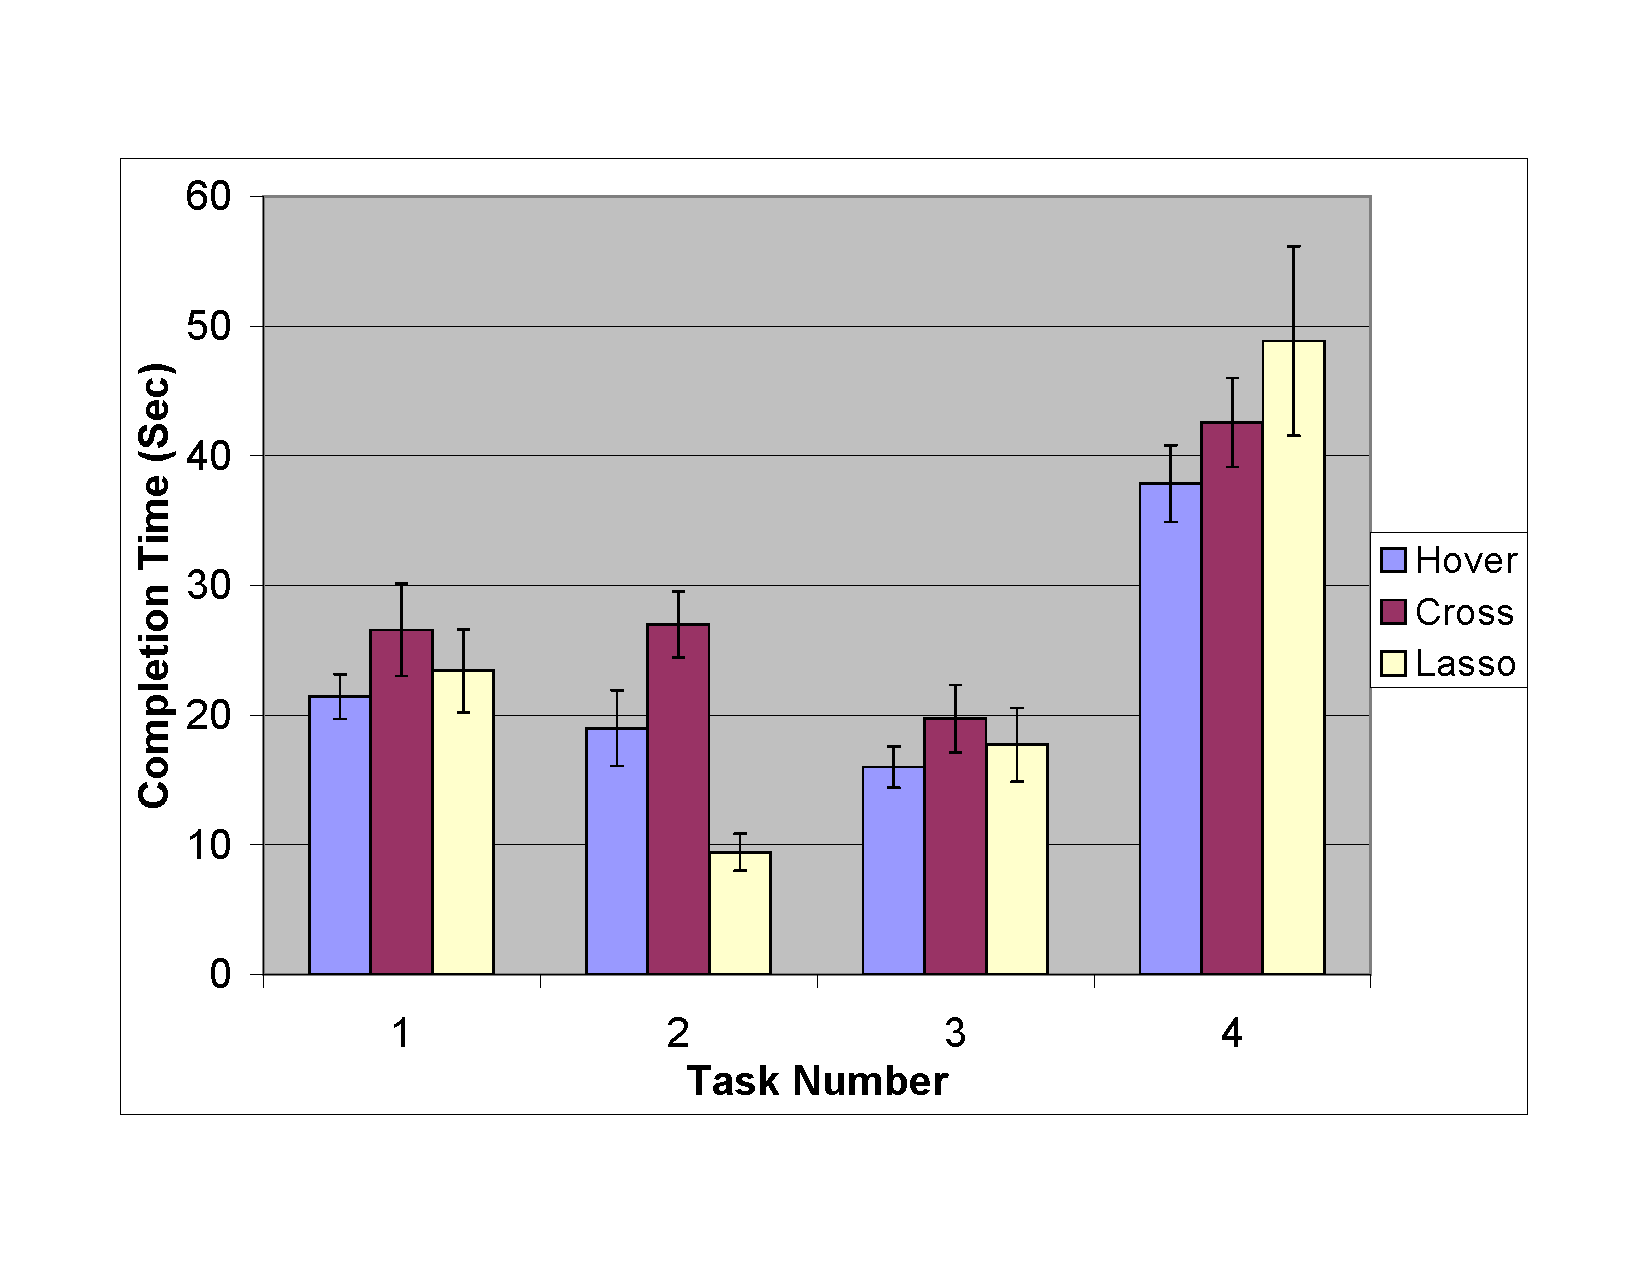
\includegraphics[width=3.0in]{results}
\caption{Average time to complete each task with each interface.}
\label{fig:times}
\end{center}
\end{figure}

Overall, users felt that it was easy and fast to select objects with
HoverCross.  Figure~\ref{fig:times} shows task completion times.  For
tasks 1, 3, and 4, we found no significant difference in completion
time between the three interfaces using a one-way within subjects
ANOVA for each task.  
For these same tasks, four users preferred HoverCross over the other
two interfaces (Figure~\ref{tab:pref}). They enjoyed the modeless
transition between sketching and selecting, without the hassle of
pressing a button or other explicit indication, despite the
reliability of the button. In addition, for small selections, drawing
a circle around the objects seemed excessive. When objects were spread
out over the canvas, they felt that selecting a few of them with lasso
select was awkward, while with HoverCross they could simply move the
pen across the screen to the objects of interest.  In fact, for this
task (number 4), although we did not see any significant difference in
completion times, for three users HoverCross much was faster than
lasso select (between 33-40\% faster).  This result suggests that
there is a set of users that would benefit greatly from HoverCross in
this situation.

\begin{figure}
\begin{center}
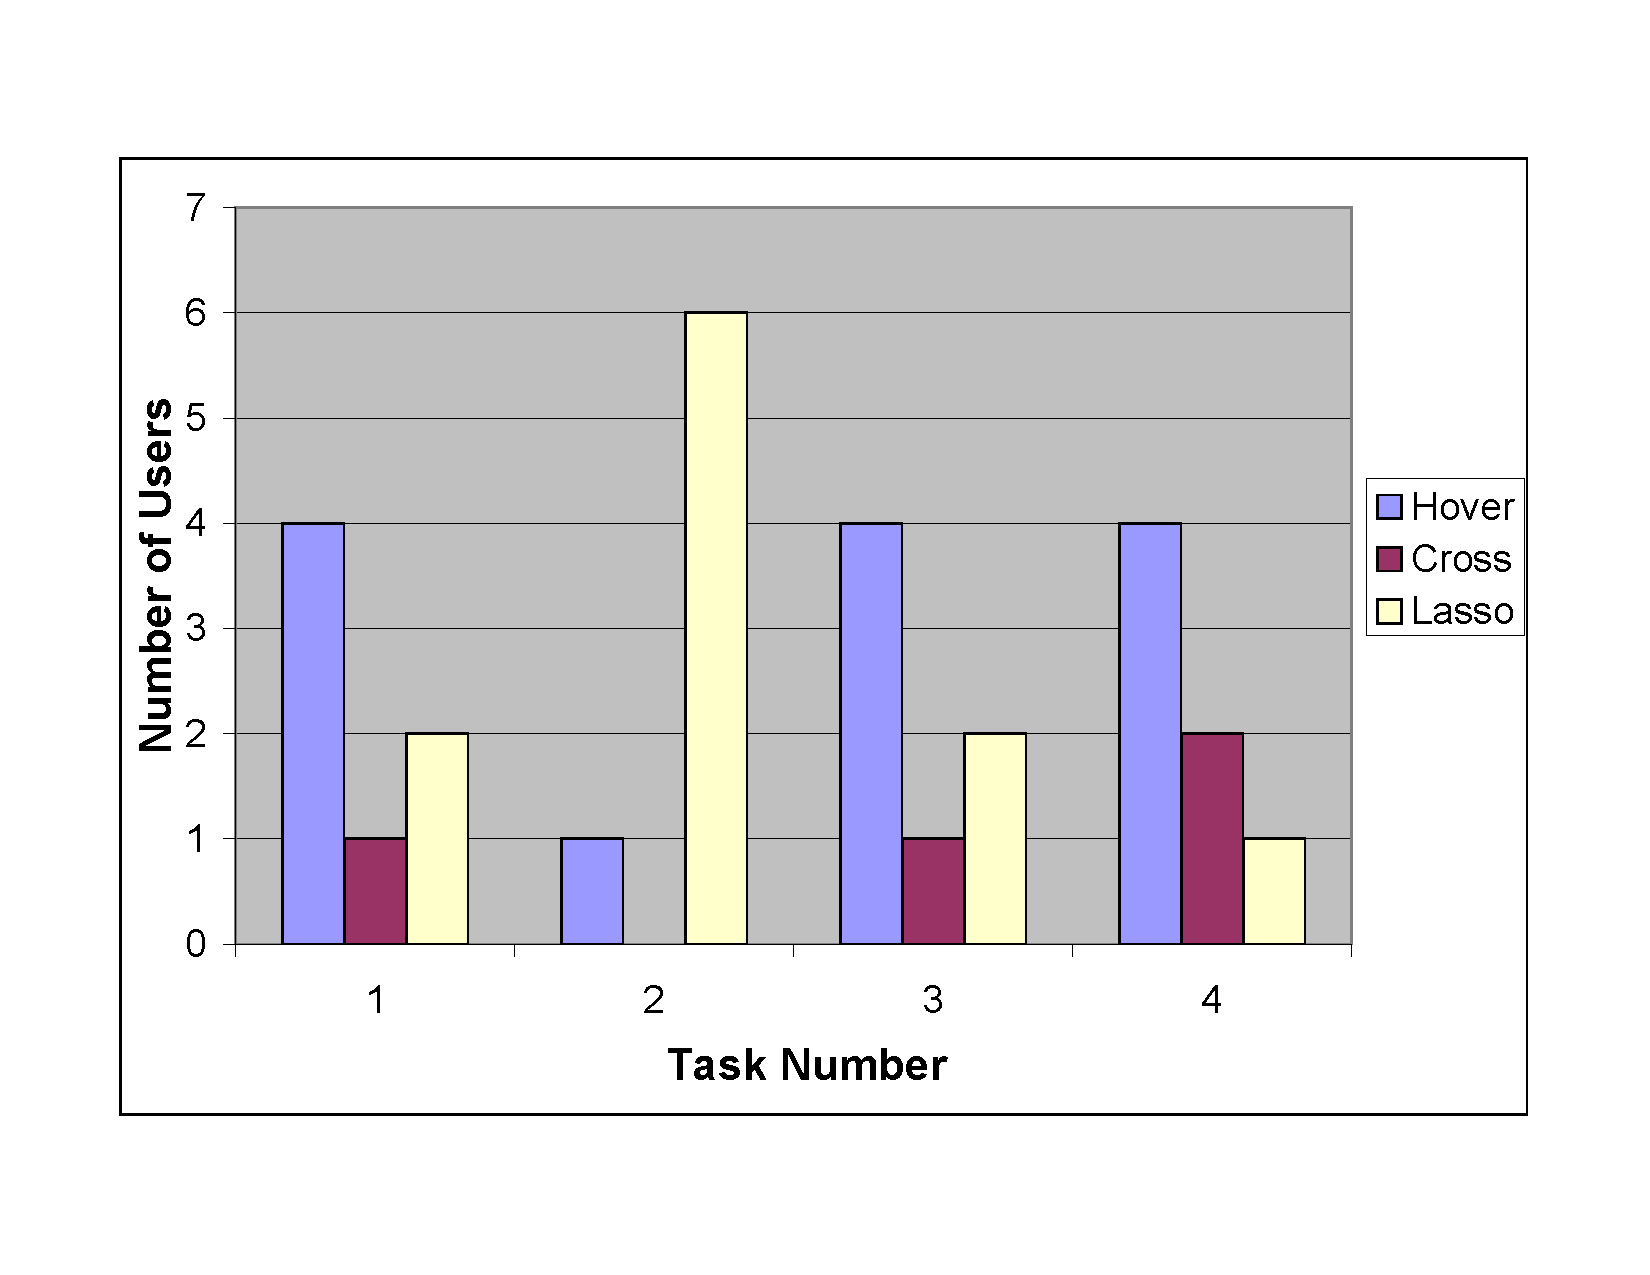
\includegraphics[width=3.0in]{Preferences}
\caption{Number of users who preferred each interface for each task.}
\label{tab:pref}
\end{center}
\end{figure}


For task 2, which involved selecting a group of closely placed
objects, six of the users preferred lasso select.  This result is
understandable, because crossing over each individual object in the
group is more cumbersome than drawing a lasso around it.  We also
found a significant difference between completion times. However, one
user still preferred HoverCross for this task.  He reflected that,
while both interfaces are effective, HoverCross was more interesting
and fun.

Although our study was small, we believe these results show great
promise for the HoverCross interface.  First, the users who preferred
the lasso select interface admitted that the most significant reason
that they preferred this interface was because of its familiarity.  We
believe that users also will get faster at using HoverCross with
practice.  Second, the general preference for HoverCross over Cross
shows the promise of using the hover space as a fluid and reliable
method for invoking selection.  Finally, while the results of task 2
show the limitations of HoverCross, we easily can combine the
HoverCross interface with a traditional button-triggered lasso select
interface to allow the user to choose the editing method that is most
appropriate for a given situation.

A number of small improvements would also make our simple prototype
even more effective.  First, the desired time lag before entering
hover select mode varies by user, so we wish to allow the user to
adjust this time.  Second, we need to optimize the specific placement
of crossing handles to deal with small objects and mostly occluded
objects.  Some users suggested that we make the selection crossing
handle and the selection indication more visible.  Finally, as our
system is only a prototype, occasionally a bug results in unexpected
behavior, such as not correctly recognizing crossing of the handle
each time.  Fixing these bugs would certainly improve the usability of
the interface.

\section{CONCLUSION}
HoverCross combines the simplest and most effective ideas from many
recent advances in pen-based interfaces to provide an elegant
interface for inking and editing.  Used in combination with other
pen-based interaction techniques, HoverCross will bring us one step
closer to the goal of creating pen-based interfaces that combine the
freedom of paper with the power of the computer in a useful, and
usable, way.  

% use \newpage to break the columns on the last page so they have equal length
% if the break occurs in the middle of a paragraph, insert \linebreak before \newpage
%\linebreak
%\newpage

\section{ACKNOWLEDGEMENTS}
We would like to thank our users who helped us evaluated HoverCross.
This work is funded by the Baker Foundation and an NSF CAREER award
(IIS-0546809).

%%%	You can use bibtex if you like, but I've hardwired in these 
%%%	references to avoid sending you a separate .bib file.
\bibliography{uist08}



\end{document}
